%=========================================================================
% (c) 2014, 2015 Josef Lusticky

\subsection{Transmit offloads}
Most of the adapters that support receive checksum offload
also support its counter-part transmission (Tx) checksum offload.
Tx checksum offload calculates TCP/UDP and
IP checksums of the packets in the hardware before they are transmitted on the wire.

A counter-part of LRO is TCP Segmentation Offload (TSO).
With a TSO-capable adapter, the kernel can prepare much larger packets for outgoing data
(e.g. up to 64KB in case of IPv4) and the adapter will re-segment the data into smaller packets according to the MTU~\cite{jls2009-gro}.
TSO is well supported in Linux -
for systems which are engaged mainly in sending of data,
it is sufficient to make 10~Gbps rate~\cite{jls2009-gro}.
TSO reduces the necessary CPU load, bus overhead, and cache impact to send a series of packets,
but it still does not require the adapter to actually know
anything about specific TCP connections -
the kernel still has to deal with the TCP states and ACKs~\cite{linux-and-tcp-offload-engines}.

The TCP Segmentation Offload is designed to work with TCP exclusively.
To mitigate this issue, the Generic Segmentation Offload (GSO) was implemented.
Performance improves even if the feature is emulated in the driver~\cite{jls2009-gro}.
Figure~\ref{fig:linux-tx-offloads} shows comparision of egress packet processing
with and without the above described offload mechanisms.
\begin{figure}
	\centering
	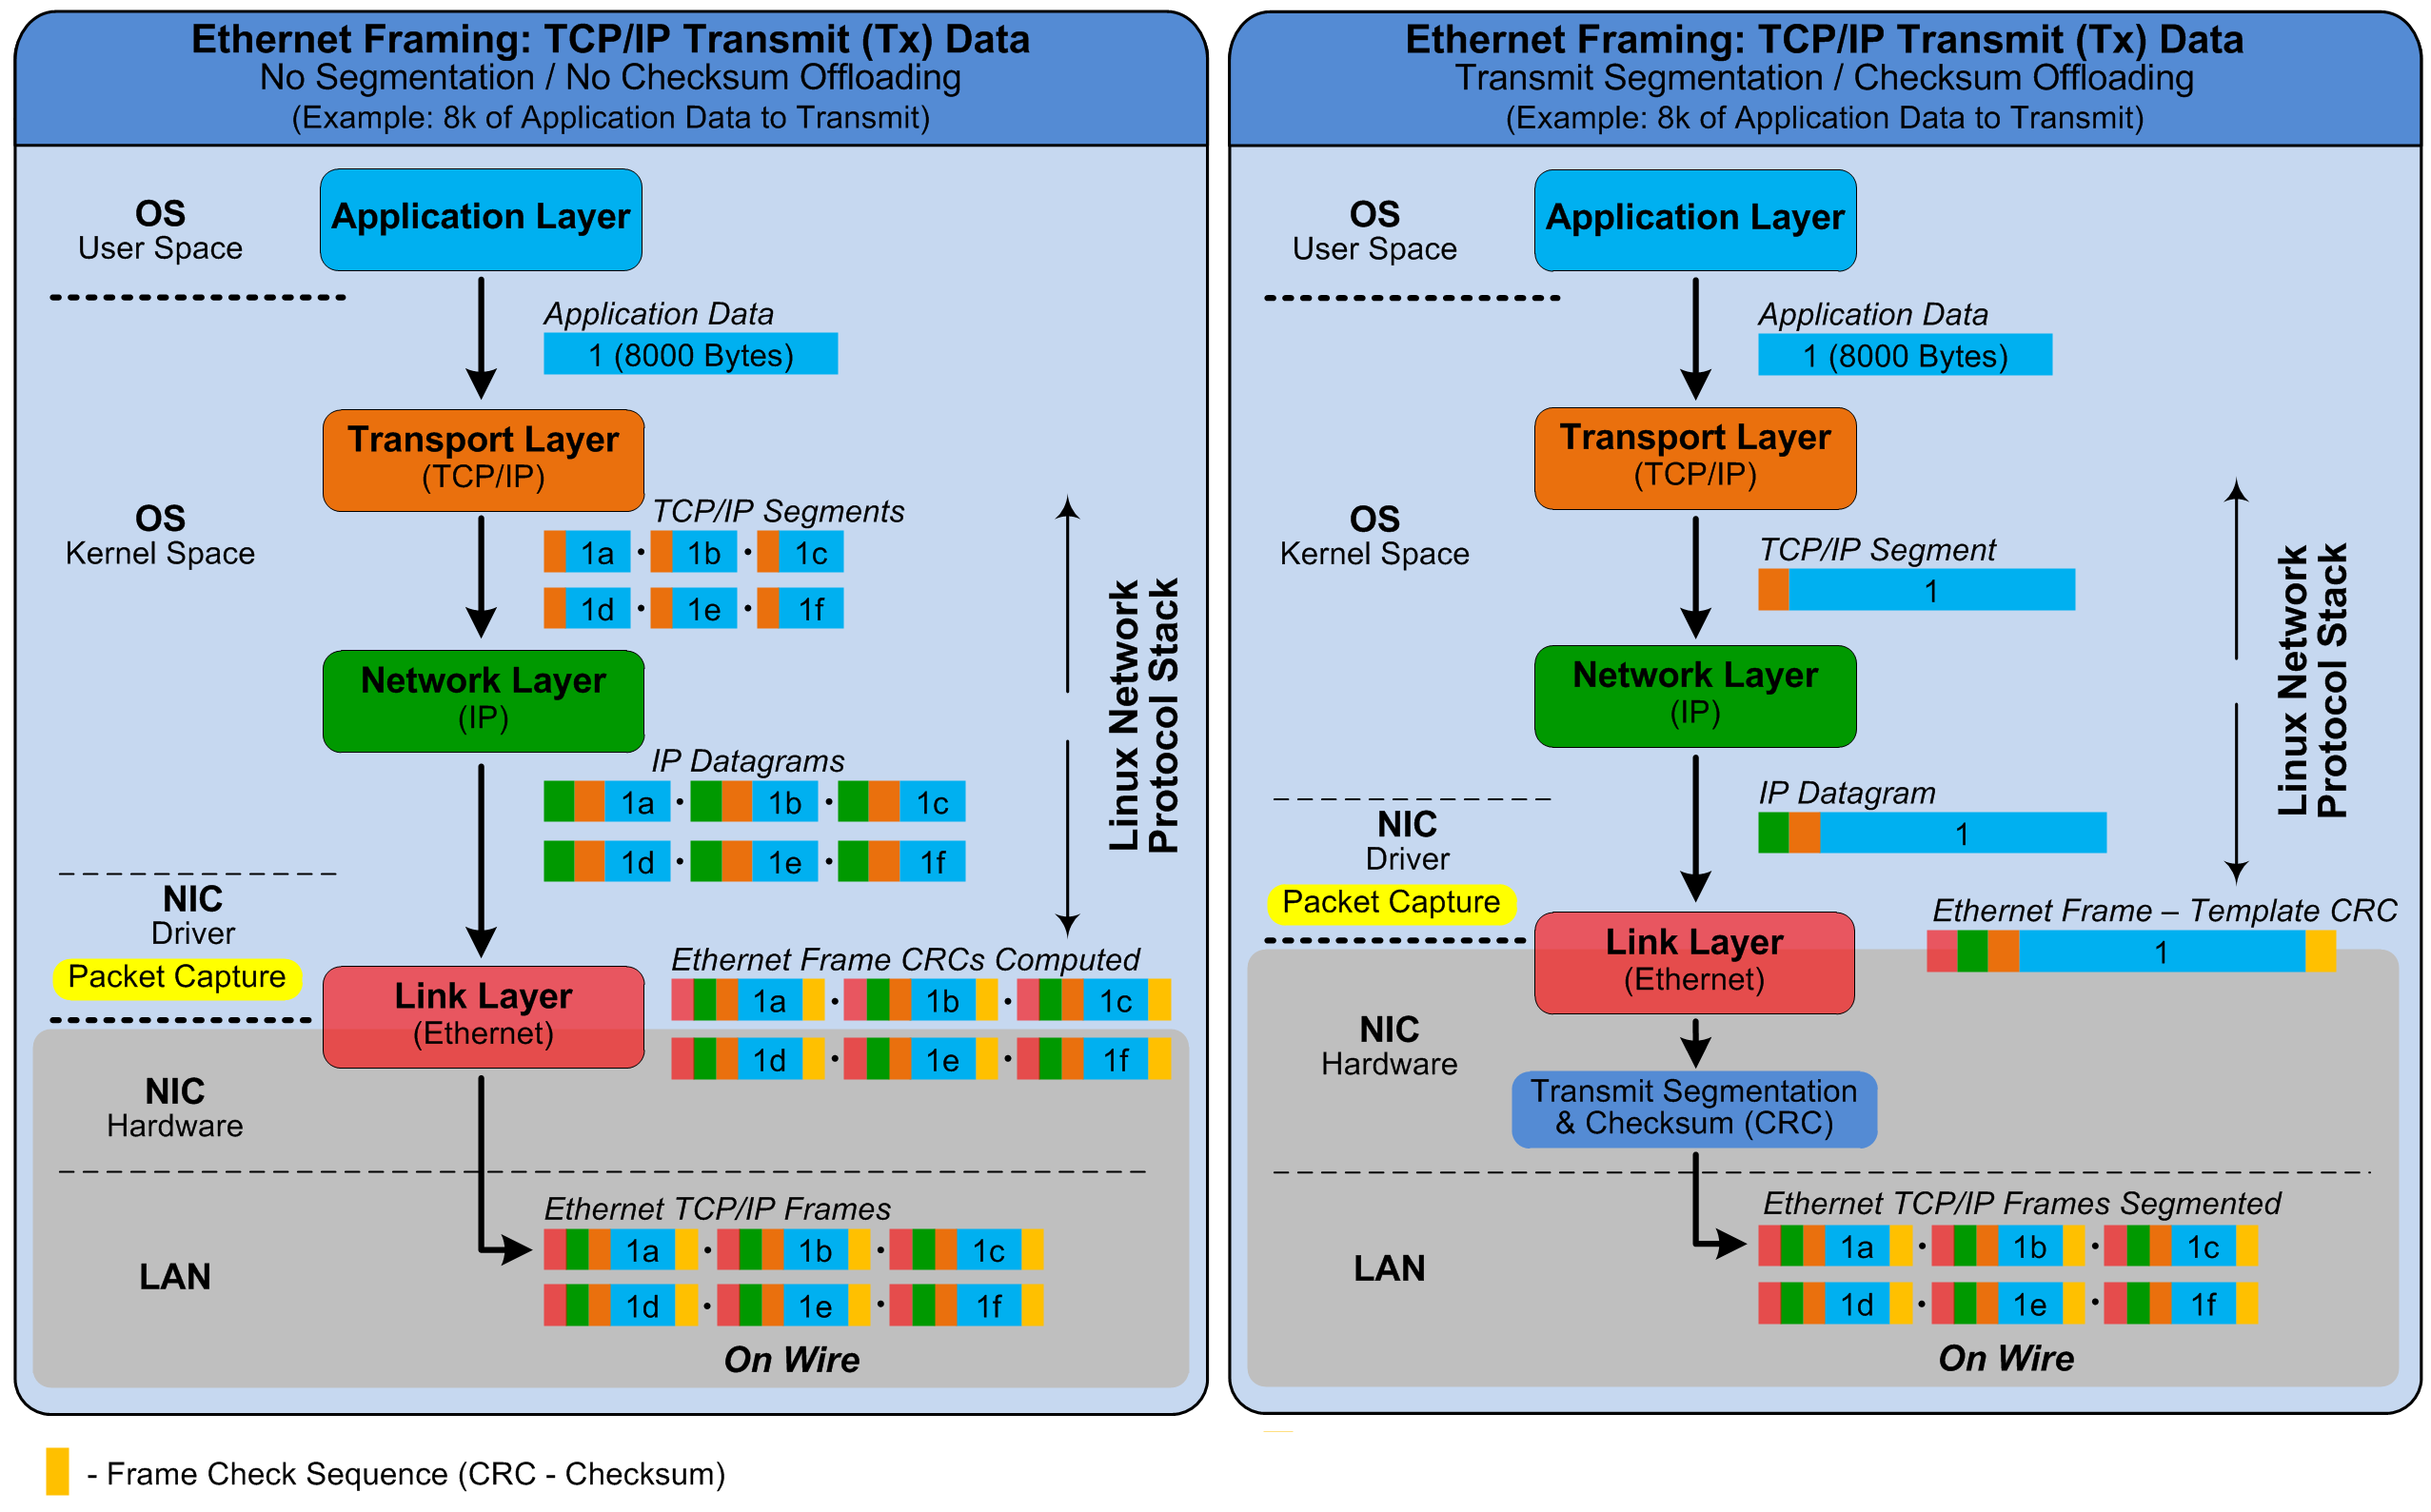
\includegraphics[width=15cm,keepaspectratio]{fig/tx-offloads.png}
	\caption{Transmit offloads (source:~\cite{nst-offloads})}
	\label{fig:linux-tx-offloads}
	\bigskip
\end{figure}
